\subsection{CIB電源系}

\begin{figure}[htbp]
	\begin{minipage}{0.5\hsize}
		\begin{center}
			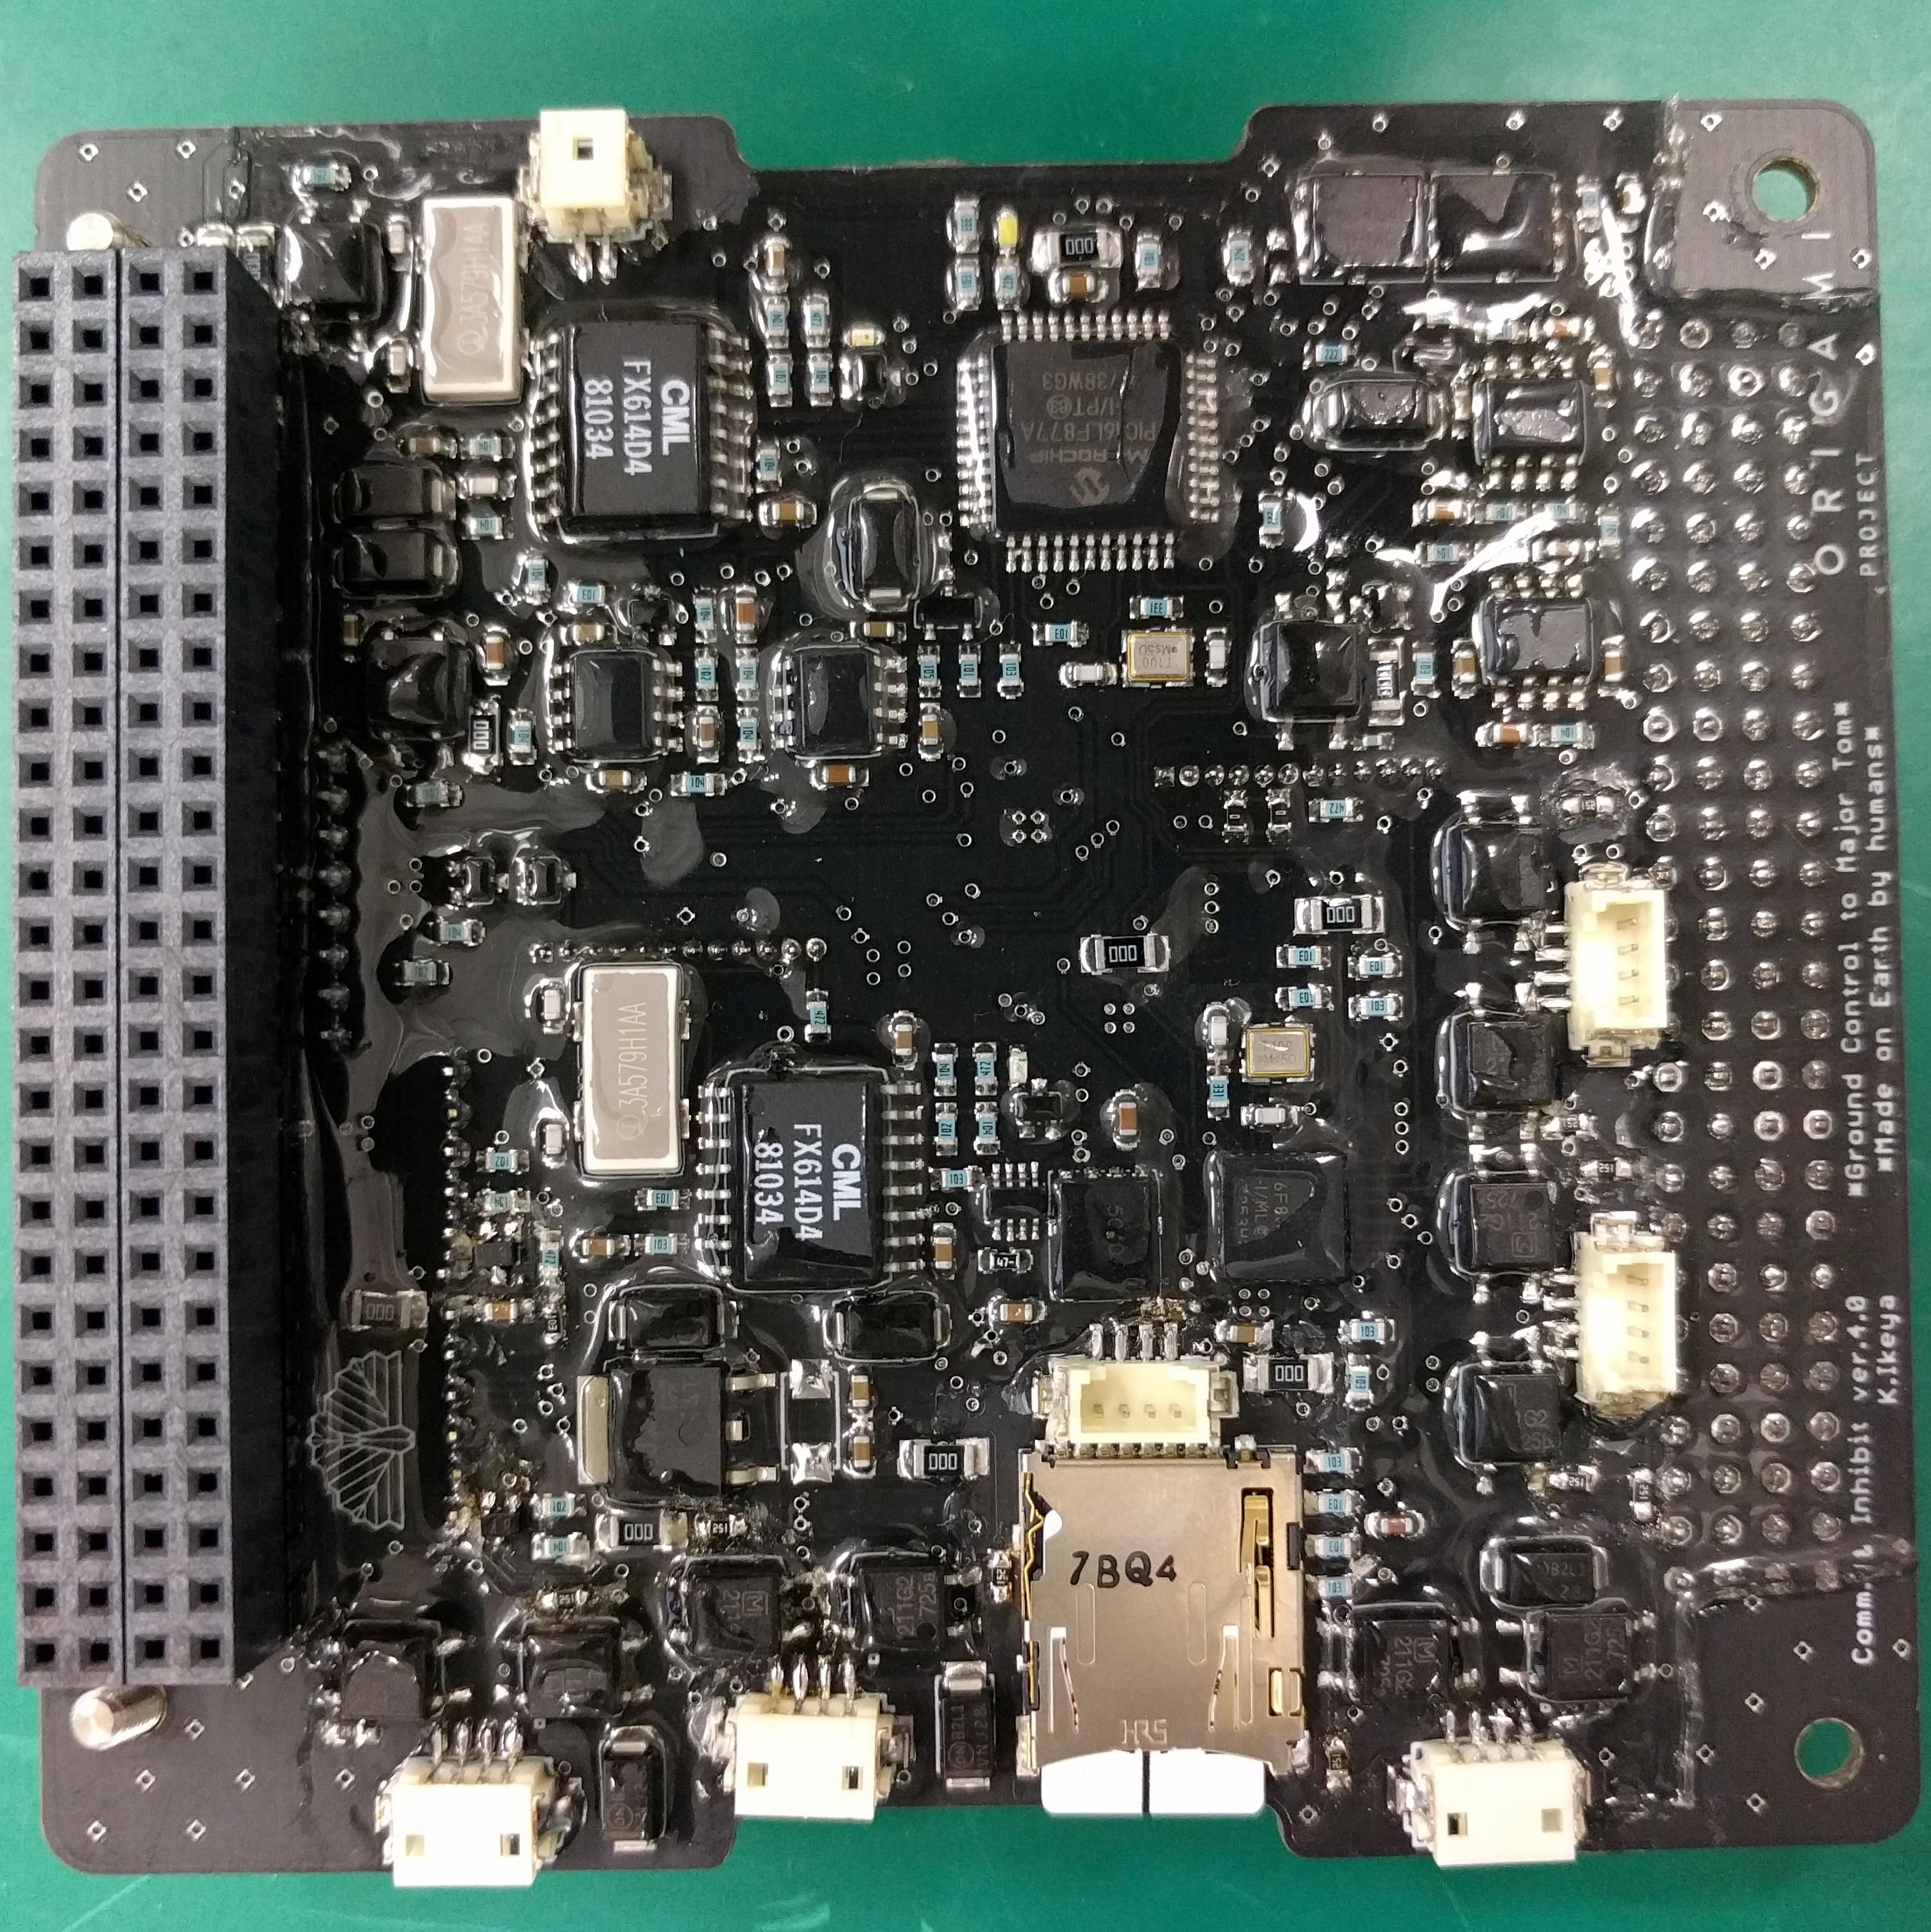
\includegraphics[width=0.7
			\linewidth]{./03/fig/CIB_1.jpg}
		\end{center}
	\end{minipage}
	\begin{minipage}{0.5\hsize}
		\begin{center}
			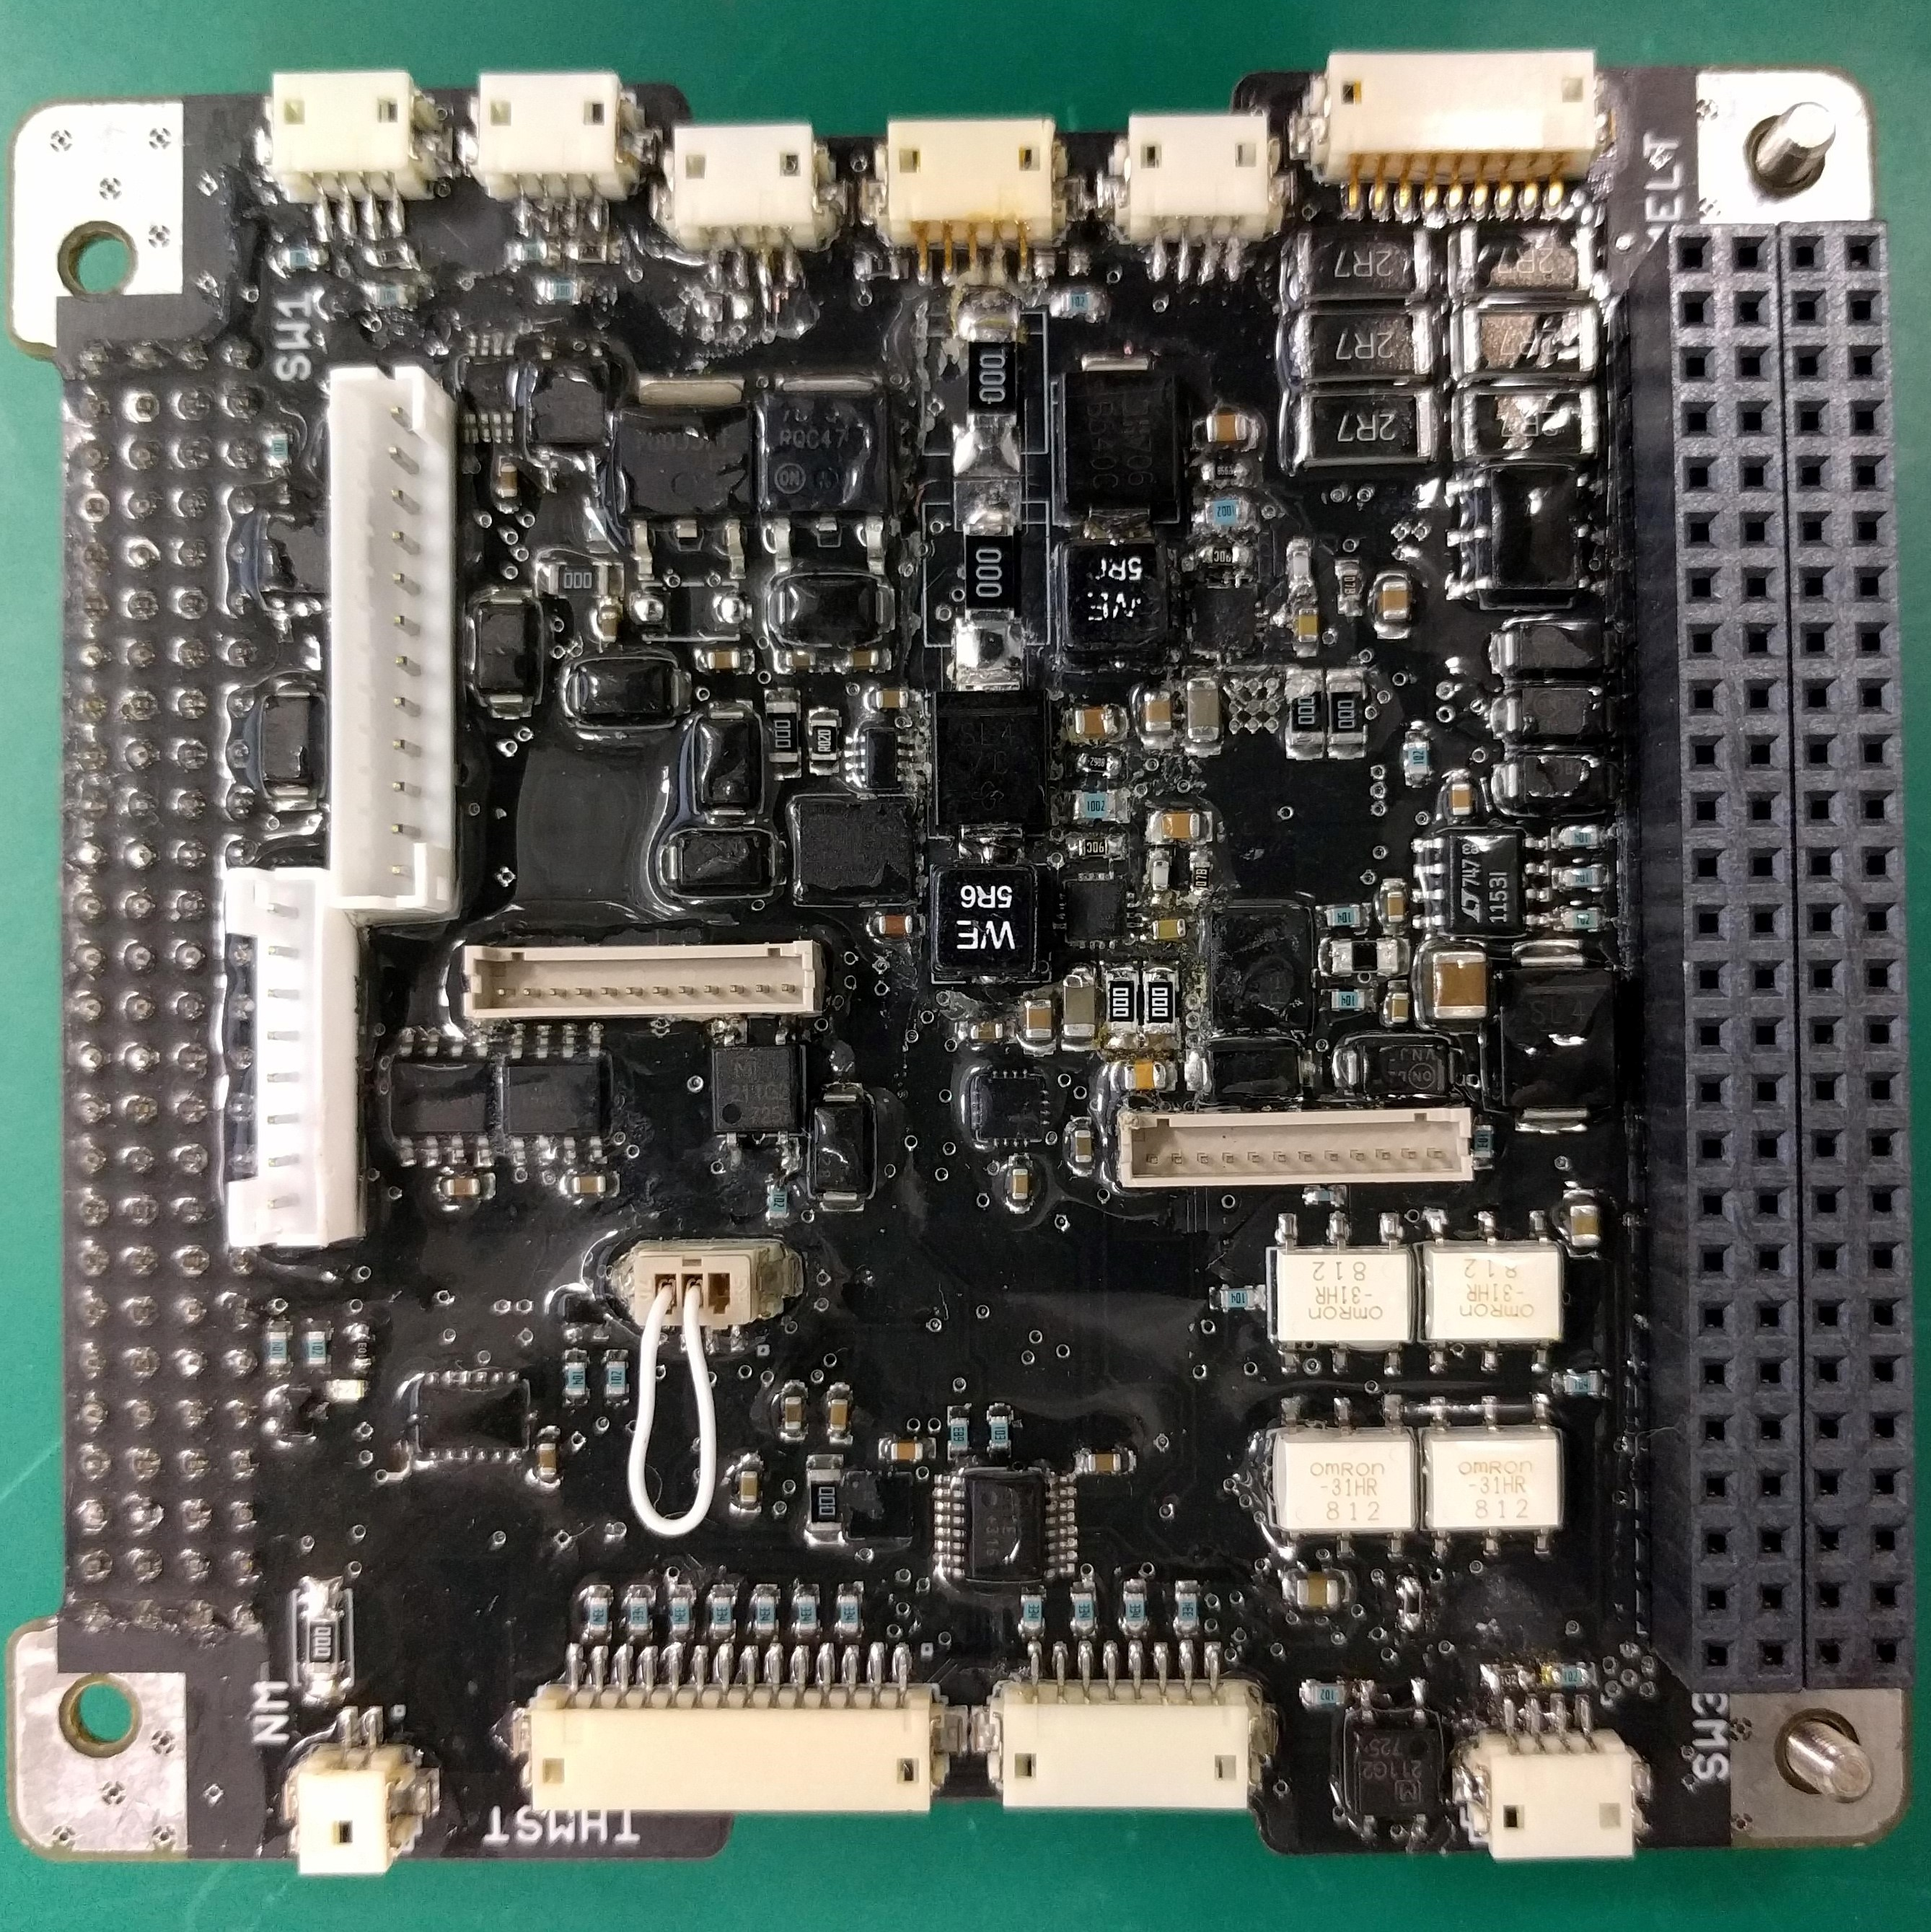
\includegraphics[width=0.7\linewidth]{./03/fig/CIB_2.jpg}
		\end{center}
	\end{minipage}\\		
	\begin{center}
		\caption{CIB}
	\end{center}
\label{CIB}
\end{figure}

\subsubsection{インヒビット回路}
イプシロンロケット
ACX-11007「小型副衛星の安全設計手引き制定初版」を参考に
要求により

以下のハザードを設けられた
これらのハザードに対応するために
3インヒビット回路を設けた.

購入品ではこれらの要求を満たせなかったため新たに

Battery-EPS間に新たに

ただし現在は3インヒビット要求を満たすバッテリがClyde Space社から新たに発売されている

\begin{figure}[htbp]
	\begin{center}
		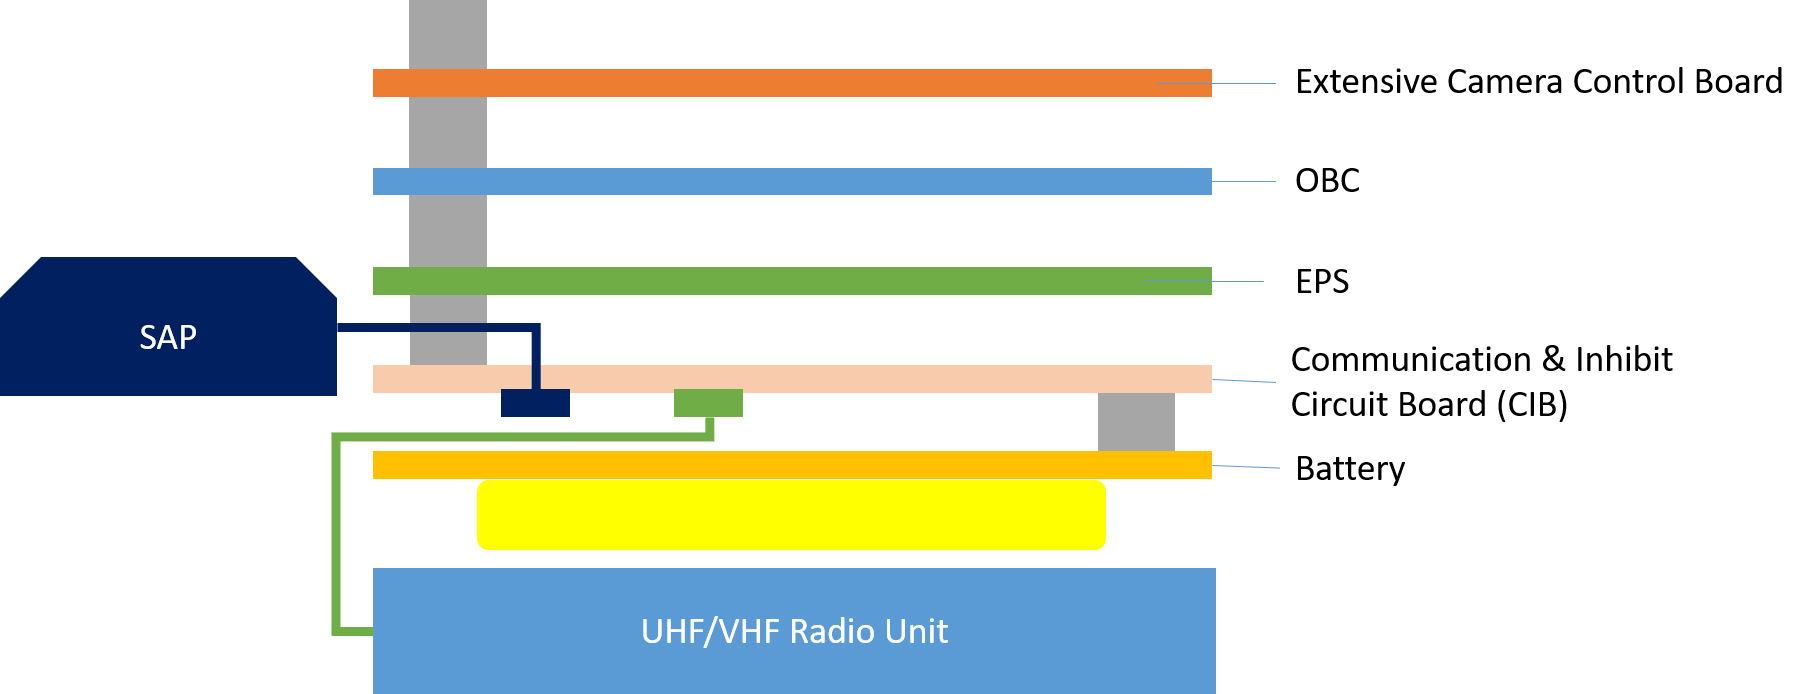
\includegraphics[width=0.7\linewidth]{./03/fig/cib_position.png}
		\caption{Cell level protection circuit schematic 転載}
		\label{fig3_1_cibposi}
	\end{center}
\end{figure}
インヒビット回路の回路図は

のようになっている

SAP-EPS間の遮断


リターン側のMOSFETをBack to Back
で双方向
実際には片方のみで問題ない
HOT側のPhotoMOSは
型番


これらのIC選定の基準として

またP-chanel MOS

回路の簡易化のために
ただしMOS
内部抵抗は概して小さい
これらのIC動作の不具合は致命的であるため
実際には並列に接続した

\begin{figure}[htbp]
	\begin{center}
		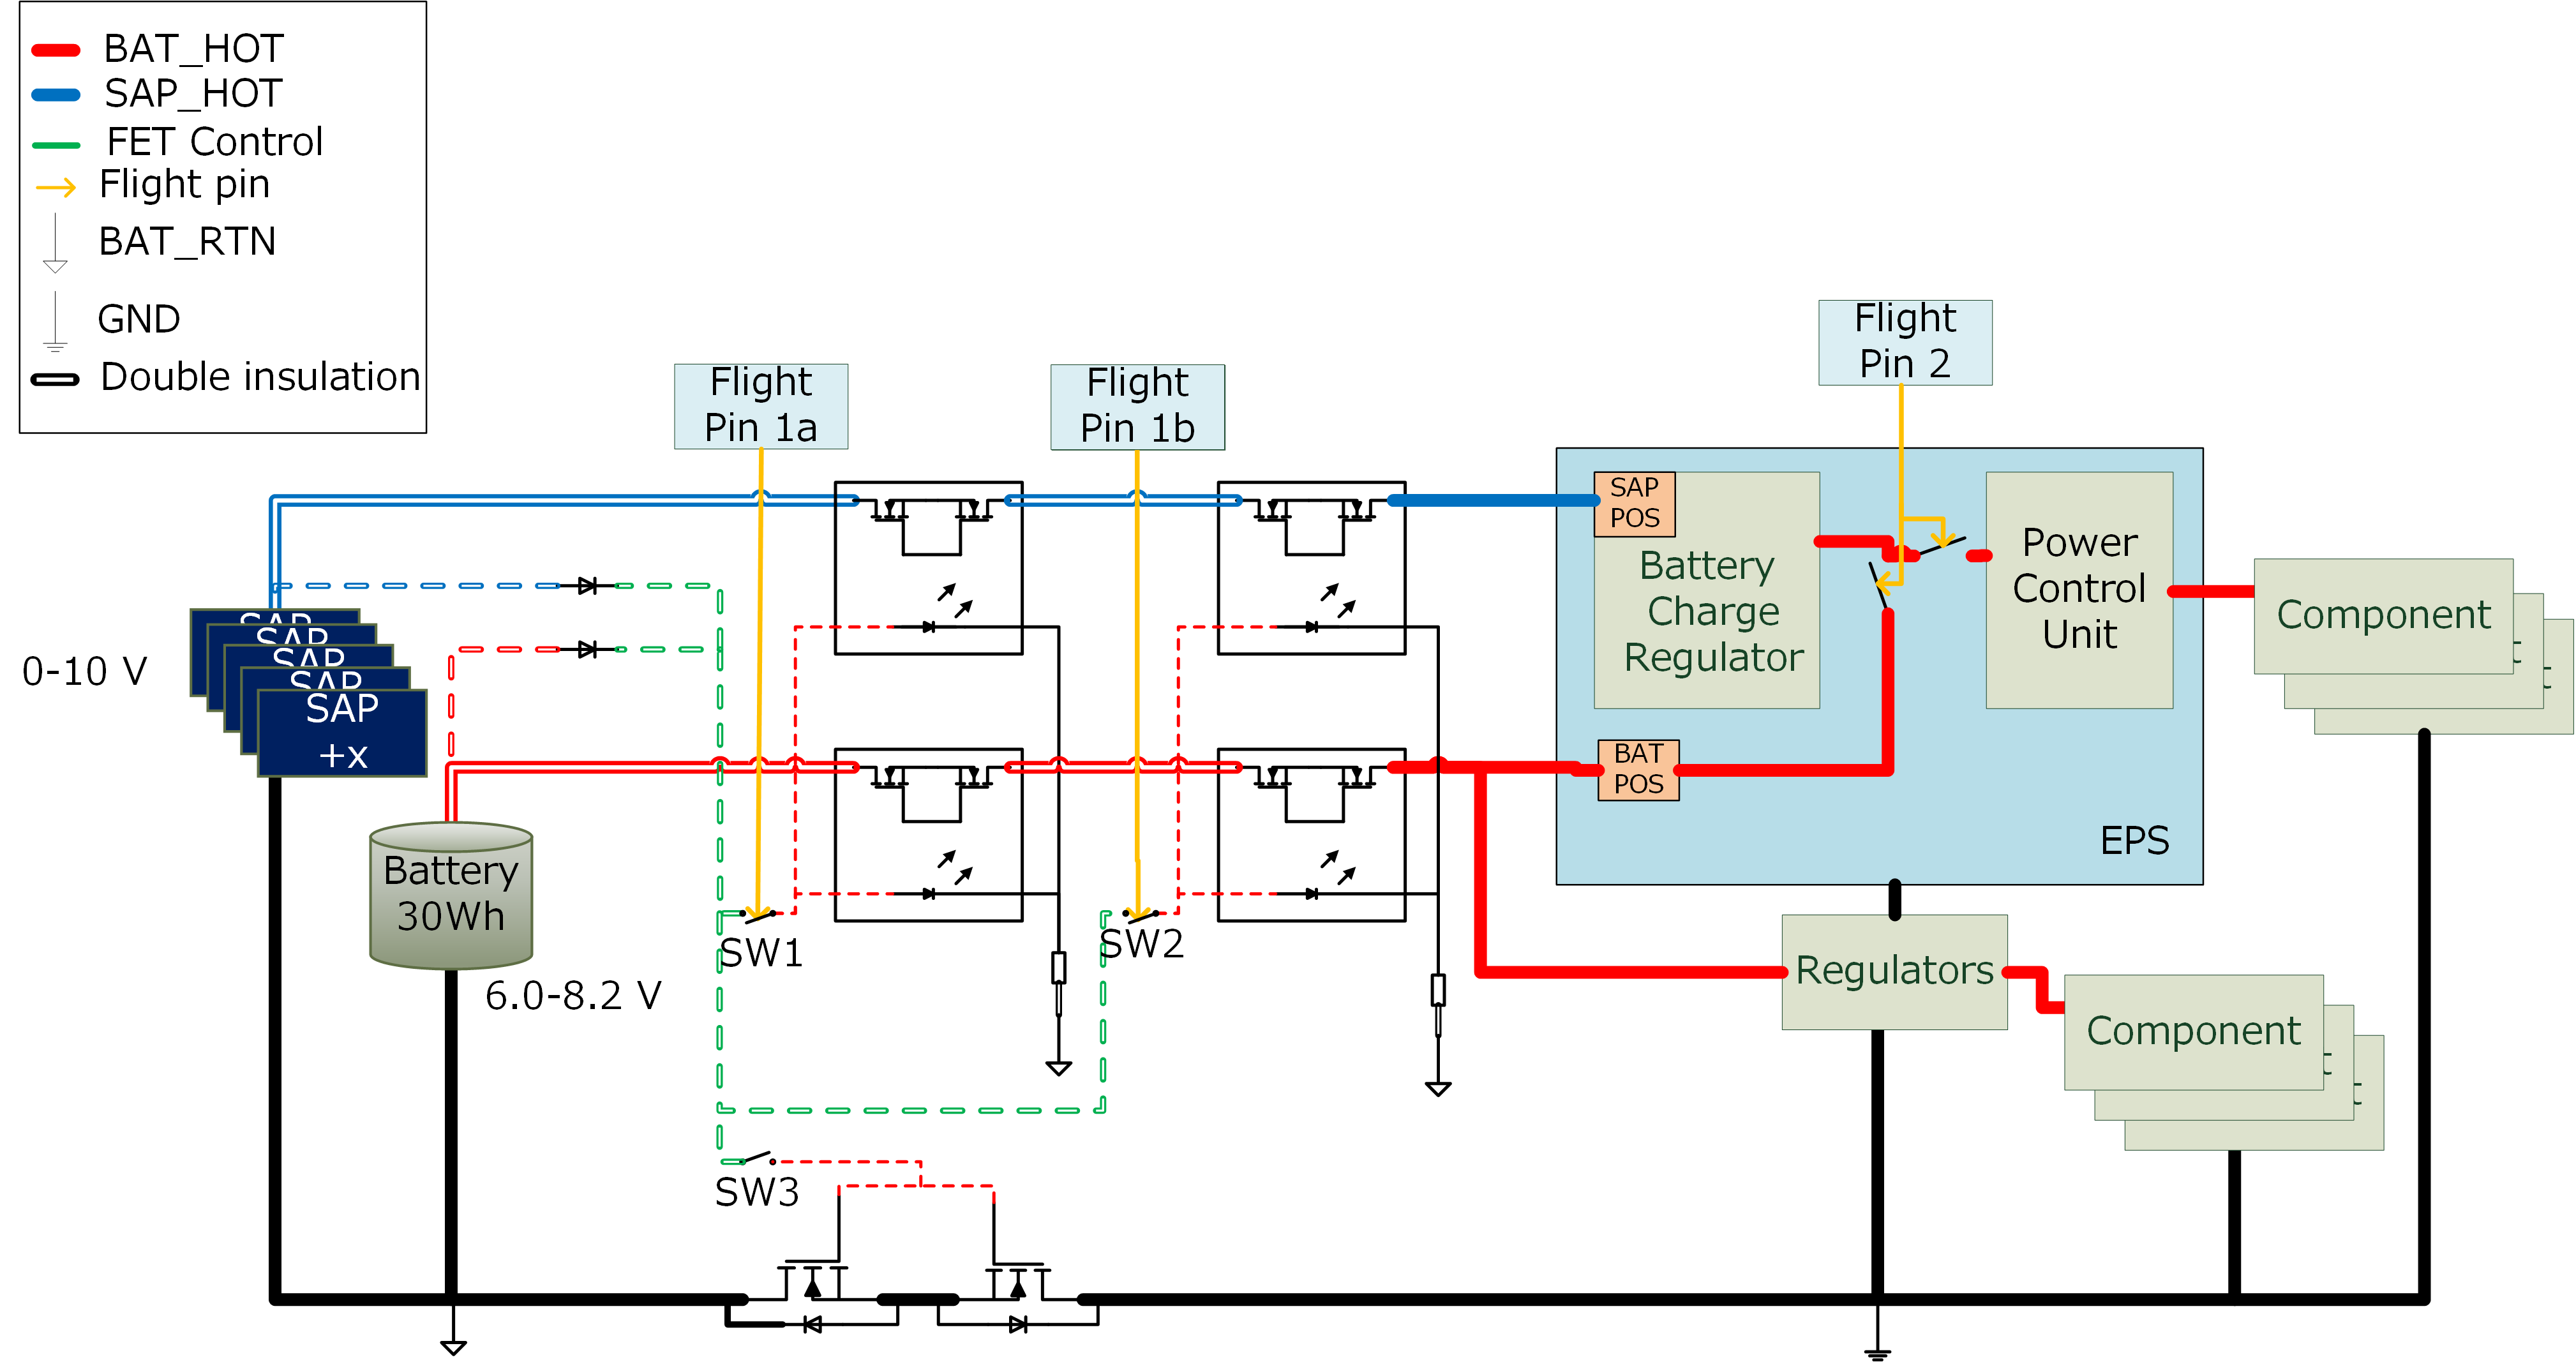
\includegraphics[width=0.9\linewidth]{./03/fig/inhibit_diagram_2.png}
		\caption{Integrated EPS and Battery Protection Architecture 転載}
		\label{fig3_1_inhibit_d}
	\end{center}
\end{figure}

\subsubsection{フライトピン}
衛星のハンドリング中




\subsubsection{CIB内電源回路}
通信用マイコンであるRXCOBC,TXCOBCはミッション開始から終了までほぼすべての期間で起動している必要がある.EPSから供給されるコンポーネントの一括on/offを可能にするためにこれらの電源系はEPS基板とは別に新たに設け,EPS電源が入っていない状態においても衛星として最低限の役割が機能するように設計した.




そこで新たな電源回路をCIB内に設けた.RXCOBC,TXCOBCの電源である3.3 V系は軌道上での故障が許されない
そこで一般的に効率の良いスイッチングレギュレータ,ではなく信頼性の高い三端子レギュレータを使用した.さらにレギュレータが1つ動作しなかった場合に備えて二つのレギュレータを並列で繋いだ.

参考文献


\begin{figure}[htbp]
	\begin{center}
		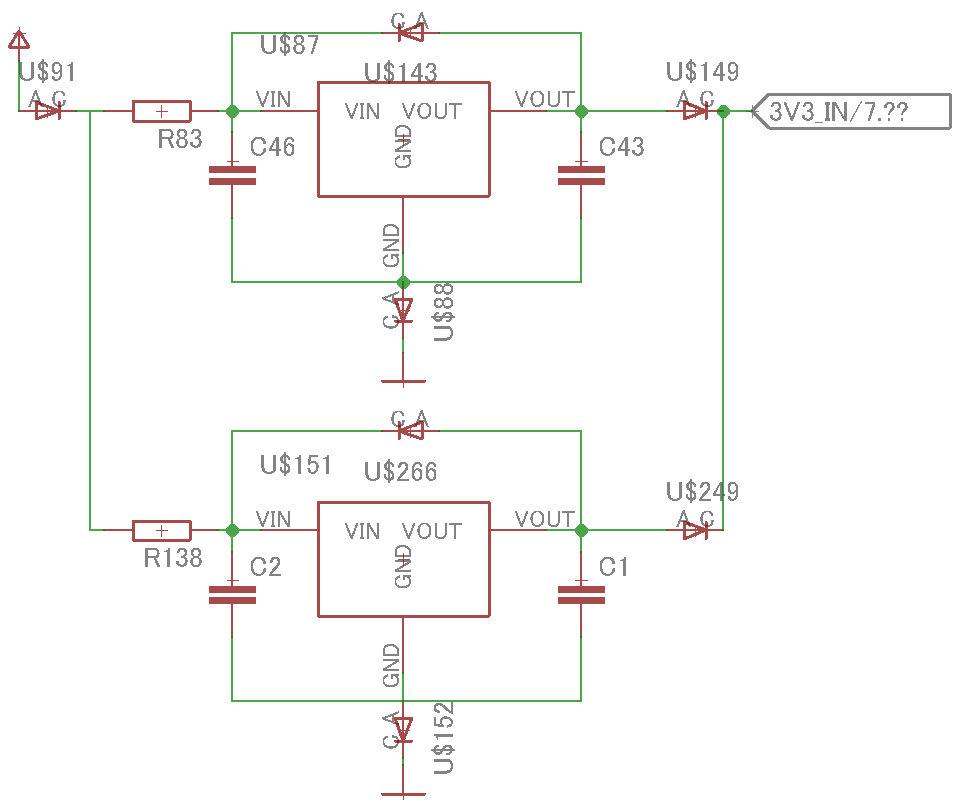
\includegraphics[width=0.6\linewidth]{./03/fig/3V3.png}
		\caption{Integrated EPS and Battery Protection Architecture 転載}
		\label{fig3_1_inhibit_d}
	\end{center}
\end{figure}

およびUHF/VHF無線機


また5.8GHz送信を行う際の突入電流が非常に大きくEPSの
保護機能が働いてしまうために12V系も新たにCIB上に設計した


12V系は
突入電流が
購入EPSの

そこで新たにDC-DCコンバータ

これらは二重に

さらに過電流対策

放射線試験によるICの放射線耐性を



